\documentclass{notube}
\usepackage{capt-of}


\WP{7c} \WPName{Internet TV in the Social Web}

\delID{7c.3} \delName{Social TV: Personal and Group Preferences, v.2}
\delNameRunning{Deliverable D7c.3} \delCoordinators{Vicky Buser (BBC),}

\delContributors{Libby Miller (BBC), Dan Brickley (VU)}

\delQualityAssessor{Dong Liu}

\delQualityController{Lyndon Nixon}

\dueContractual{M33}
\dueActual{31-10-11}
\status{0.8}

%\final

%\prototype
\report
%\dissemination

\public
%\consortium

\authorPartner{Vicky Buser (BBC),  Libby Miller (BBC),  Dan Brickley (VU)}
\responsibleAuthor{Vicky Buser (BBC)}
\responsibleAuthorPartner{BBC}
\responsibleAuthorEmail{vicky.buser1@bbc.co.uk}
\responsibleAuthorPhone{+44 (787) 6565561}

\summary{
The main objective of this deliverable is to provide an overview and update of the work in workpackage WP7c ``TV and the Social Web”, with a particular focus on user experience. It also sets out to place this work in the wider context of developments in Web and TV convergence outside the project.

During Years 1 and 2 of the project we focused on laying the foundations for building useful and user-friendly social TV applications by creating an infrastructure based on re-usable APIs and the use of URLs to identify programmes to disambiguate specific episodes. We also developed several prototypes for exploring ways of finding something interesting to watch, finding out more about a programme, having online conversations and sharing emotional reactions to a programme.

During Year 3 we have further developed the most compelling aspects of these prototypes and extended the use cases to consider scenarios involving small groups of people watching TV together, both in the same room and remotely, with each individual having their own second screen device. This work has culminated in `N-Screen’, an html/javascript multi-screen demonstrator for real-time collaborative browsing and sharing of programmes and for changing the TV display. N-Screen is a flexible framework that can be adapted for different data and content sets, and to integrate different combinations of recommendation strategies developed in the project. Alongside N-Screen we have also been considering collaborative annotation of video for second screen experiences with our TV Extras Authoring (TEA) and TeaPlayer demos.

We still consider the second screen to be a personalised extension of the TV experience and we recognise the importance of creating a good user experience. Therefore, earlier this year we worked with a group of Masters students at the VU to explore usability heuristics for TV second screens, producing some draft guidelines which we hope that creators of second screen apps can re-use and build upon. We also developed and integrated more polished and professional user interfaces for N-Screen in time for IBC and for the purposes of user testing.

We have continued to monitor relevant developments outside NoTube, where we have seen an extension of previous behaviours around increased social media usage combined with TV viewing, the predominance of second screen experiences, and increasing interest in data mining of activity and social data for the provision of social recommendations. These are all trends which are reflected in our work.
}

\abstract{
During Year 3 of the NoTube project, in workpackage 7c ``TV and the 
Social Web" we have been consolidating the work of previous years 
by developing the `N-Screen’ demonstrator framework for exploring 
the key themes of content discovery, sharing within small groups, and 
use of multiple personalised second screens in conjunction with a 
shared TV. We have also been exploring collaborative annotation of 
video content with the TV Extras Authoring demo (`TEA’). 

We believe that good user experience is crucial in determining the 
future direction of TV. This is why we are intending to devote a substantial 
amount of time during the rest of the NoTube project to user testing of 
N-Screen and of comparing second screen with single screen experiences.
}

\keywords{
}

\versionLog{
    \versionLogEntry{\today}{Vicky Buser}{0.8}
}


\begin{document}

\maketitle

%\include{abbreviations}

\chapter{Introduction}

The main objectives of this deliverable are to:

\begin{itemize}
\item{Provide an overview and update of the work in workpackage WP7c ``TV and the Social Web".}
\item{Focus on the importance of good user experience.}
\item{Place our work in the wider context of Web and TV convergence.}
\end{itemize}

During this last year we have been consolidating the work in Years 1 and 2 by developing the `N-Screen' demonstrator framework for exploring the key themes of content discovery, sharing within small groups, and use of multiple personalised second screens in conjunction with a shared TV. As we predicted in our previous deliverable 7c.2, we have also been exploring collaborative annotation of video content with the TV Extras Authoring demo (`TEA').

\begin{figure}[htbp]
\begin{center}
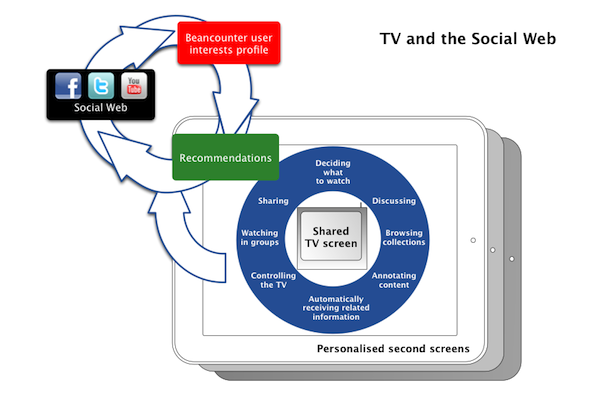
\includegraphics[width=6in]{images/summary.png}
\caption{Summary of the ideas in workpackage 7c} \label{fig:summary}
\end{center}
\end{figure} 

\chapter{N-Screen}

The scenario driving N-Screen imagines a small group of people together in the same room, each with their own personal device, deciding what to watch together on one shared TV. Alternatively the people in the group could be physically remote; in which case we assume that they are also communicating with each other using an existing chat client such as Skype or IRC.

Each participant starts with a different set of personalised recommendations from the video collection. Participants can share programmes of interest with each other and change what’s playing on the TV. Again, we assume that there are conversations taking place around the suggestions (either via the chat client or face-to-face if the participants are in the same room), providing the relevant context by explaining the reasons why a particular suggestion has been made  - ``I know you love this actor!" or ``We watched the first episode of this and it was great – do you remember?"
\footnote{We illustrated these, and other scenarios relating to the work in workpackage 7, in the latest set of NoTube postcards: \url{http://www.flickr.com/photos/nicecupoftea/sets/72157627601924949/}}

The html/javascript N-Screen multiscreen demonstrator framework allows us to:

\begin{itemize}
\item{Experiment with different data sets of on-demand content, including both long-form and short-form (for example: BBC iPlayer data, BBC programmes data, and TED talks data).}
\item{Integrate different recommendation and browsing strategies, including those based on Beancounter profiles, into one unified end-user interface. This provides multiple ways of helping people to find something interesting to watch, across the spectrum from cold-start to fully personalised.}
\item{Explore real-time collaborative browsing and social recommendations with the ability to drag and drop programme suggestions to a group or to specific individuals, and likewise to receive suggestions from friends.}
\item{Integrate other second screen functionalities such as displaying related information from the Web about the current programme (e.g. using our TEAPlayer demo which is explained in the next section), and changing the TV display.}
\item{Extend the use of XMPP (Jabber) ad-hoc group chats in the backend to support the social aspects.}
\end{itemize}

In response to reviewers’ comments in the Year 2 NoTube Review report, over the last few months we have been working with visual designers to develop a more professional and attractive visual design for N-Screen, which was implemented in time for IBC. 

We wanted to make it easier for people to browse the recommendations and to understand how they are related to each other. So we focused on how to improve the presentation and layout of the different types of recommendations: personalised (based on a user’s Beancounter profile), recommendations based on collaborative filtering extending out from each personalised recommendation, and recommendations suggested by friends. We also needed to retain the `history’ functionality to enable users to easily get back to previously viewed items. 

\begin{figure}[htbp]
\begin{center}
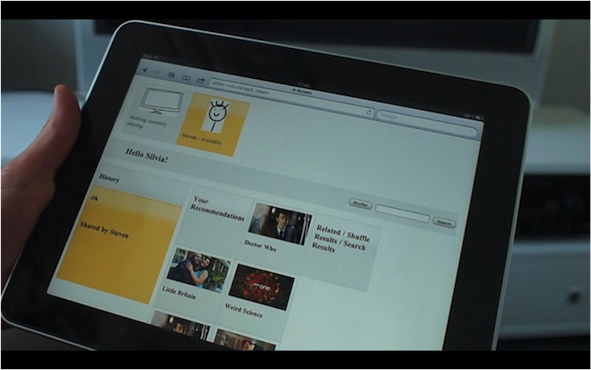
\includegraphics[width=6in]{images/ns_original.png}
\caption{Original N-Screen user interface} \label{fig:nsoriginal}
\end{center}
\end{figure}

 We achieved these goals by implementing three horizontal `streams’ for browsing: ``Suggestions for you”, ``Shared by friends” and ``Recently viewed” on the main ``browse programmes” screen. 
 
 \begin{figure}[htbp]
\begin{center}
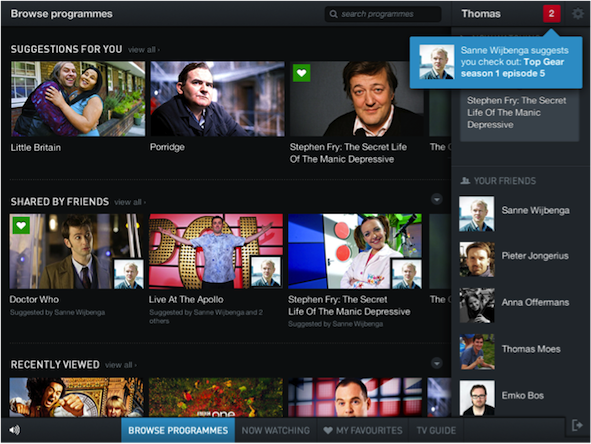
\includegraphics[width=6in]{images/ns_new.png}
\caption{New visual design for N-Screen} \label{fig:nsnew}
\end{center}
\end{figure}

Clicking on a suggestion displays an overlay with further information about the item, an explanation as to why it has been recommended\footnote{In the example shown in Figure 3, the user can see the connection between their previous activity (collected by the Beancounter) – watching the movie `Alice in Wonderland’ - and this programme.}, and a list of related programmes, based on ``People who watched this programme also watched these programmes…” The idea here is to expand out the selection of potentially interesting programmes for the user, because the list of personalised programmes could be quite small.

\begin{figure}[htbp]
\begin{center}
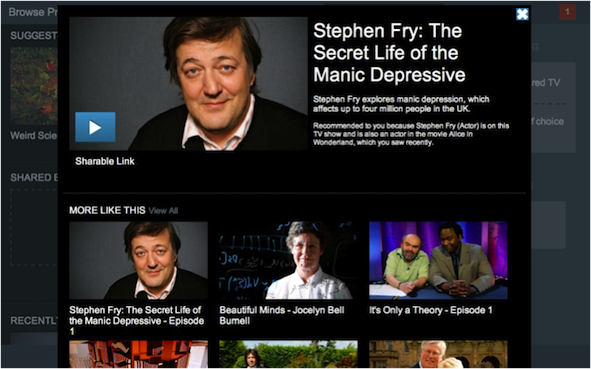
\includegraphics[width=6in]{images/fry.png}
\caption{New visual design for N-Screen programme details, displaying the programme synopsis, an explanation for the recommendation, and related programmes} \label{fig:fry}
\end{center}
\end{figure}


We were keen to keep the playful `drag and drop’ functionality (and the accompanying swooshing noise) to change the TV display and to share recommendations with N-Screen friends, which remains a highlight of the user experience. 

\begin{figure}[htbp]
\begin{center}
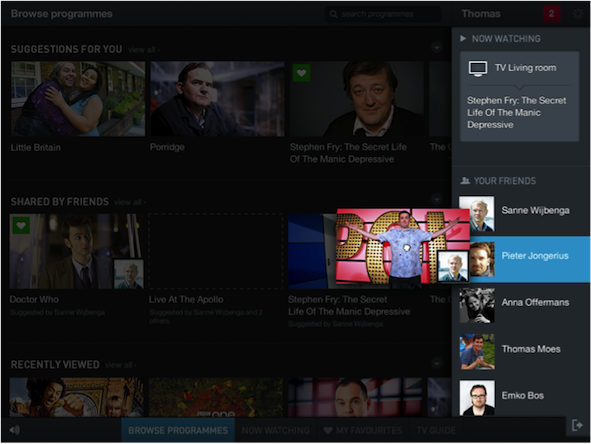
\includegraphics[width=6in]{images/dd.png}
\caption{Drag and drop in the new N-Screen design} \label{fig:dd}
\end{center}
\end{figure}

We also thought it was important from a user experience perspective to provide a ``random selection” (or ``shuffle”) option as an alternative means of surfacing content buried in the video collection, or for times when the user might reach a dead-end with the recommendations approach. 

\begin{figure}[htbp]
\begin{center}
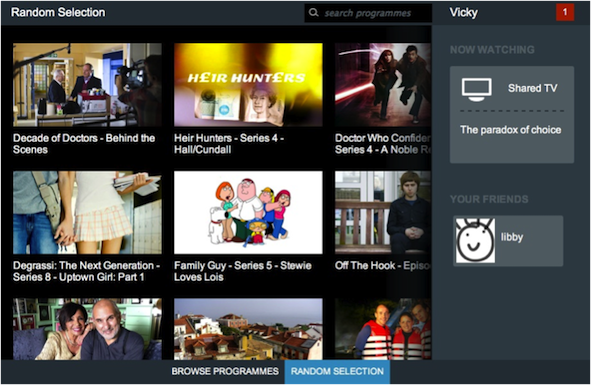
\includegraphics[width=6in]{images/random.png}
\caption{New N-Screen design showing a random selection of programmes to browse} \label{fig:random}
\end{center}
\end{figure}

The idea of showing users a random selection of items to provide another route into the content was based on the findings of our user evaluation study of the NoTube Archive Browser (the demo is described in Section 4.1 of our previous deliverable D7c.2), which we conducted earlier this year. We presented the results of this trial at the 2nd Project Review in May. 

To re-cap, we wanted to test how well re-using the BBC subject classification system, Lonclass, to present content-based links for browsing between similar programmes helped people to find interesting new programmes. Our hypothesis was that seeing similar programmes (calculated using a Tanimoto coefficient) together with Lonclass subject category information would be optimal for serendipitous content discovery. However, statistical analysis of the quantitative data we collected from the 96 participants (playlist length and the time spent browsing the video collection) coupled with the results of the online questionnaire (summarised in Figure 7 below) suggests that people enjoyed the experience and found interesting new programmes regardless of whether they saw similar or random programmes. 

\begin{figure}[htbp]
\begin{center}
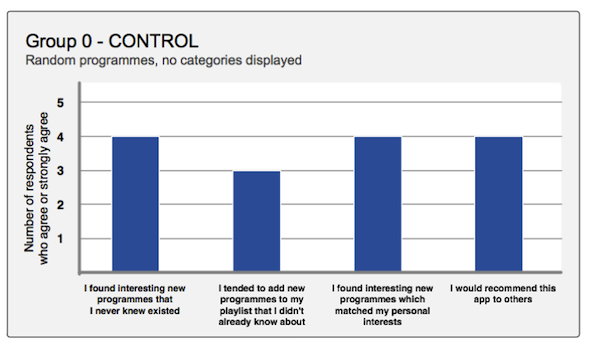
\includegraphics[width=6in]{images/group0.png}
\label{fig:group0}
\end{center}
\end{figure}

\begin{figure}[htbp]
\begin{center}
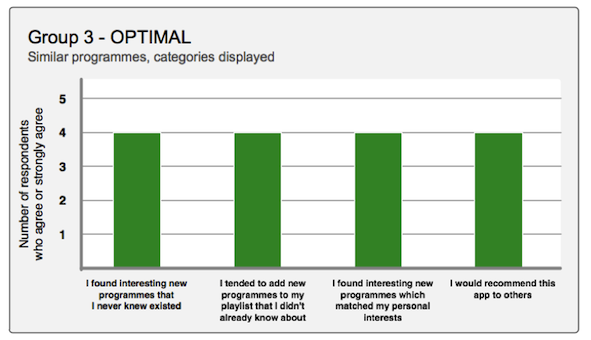
\includegraphics[width=6in]{images/group3.png}
\caption{Comparison of the NoTube Archive Browser survey results for our optimal and control conditions - showing little variation in participants' responses} \label{fig:group3}
\end{center}
\end{figure}

More details about this trial can be found on the NoTube website.\footnote{\url{http://notube.tv/2011/07/01/finding-interesting-new-programmes-trial-results/}}

\chapter{TEA `TV Extras Authoring' and TEAPlayer}

TEA is a prototype for collaboratively annotating video by dragging and dropping links to different times in the video. The usecases we considered are as follows: 

\begin{itemize}
\item{People inside a content-producing organisation are given the task of creating some second screen content for a science programme for public consumption on a second screen, with a tight deadline.}
\item{People watching a political programme use their expertise to find relevant content related to the comments made by the participants (for example Hansard text, other writing and speeches).}
\end{itemize}

`TV Extras' are like DVD Extras, specifically, content related to a video. TEA lets you author basic extras for the second screen, as you watch a video, using drag and drop from searches of the web. Two or more people can see each others' input and review it. Either can then sync the video for playback, so they can review it together. Finally, they can save their work to an intermediate file format for playback on other devices. TEA uses the same underlying infrastructure as N-Screen, although it's a bit more complex as it has state.

\begin{figure}[htbp]
\begin{center}
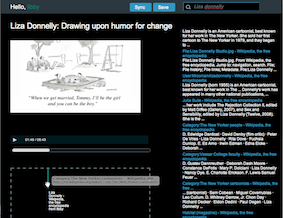
\includegraphics[width=6in]{images/tea.png}
\caption{`TEA' (TV Extras Authoring)} \label{fig:tea}
\end{center}
\end{figure}

Related to this, TEAPlayer is an experimental iPhone application built with Phonegap to play the output of TEA on XBMC. The idea was to see if the information in the file format produced using TEA could be made into a useful tool. The result is an iPhone application that looks for XBMC (a video player) instances on the same network, and allows you to choose from a selection of videos on an iPhone to play on it. If you choose an annotated video, it loads the urls on the iPhone at the correct time during playback. It also enables you to pause and play the currently playing video. 

\chapter{Setting our work in context}

The integration of the Social Web and TV continues apace towards the goal of creating more social TV experiences, including personalised recommendations based on friends’ tastes and opinions. There seems to be a shared assumption that people respond better to recommendations made by people they know\footnote{\url{http://www.guardian.co.uk/technology/appsblog/2011/sep/22/facebook-f8-social-mobile-panel}}, and this has become a core driver for major players including Facebook and Google, so that `social’ is taking centre stage in tackling the challenges of effective content discovery\footnote{\url{Despite the associated privacy issues, some of which we explore in workpackage 3}}. This is related to the role of serendipity in helping people to discover new, enjoyable things that they would probably not have discovered on their own, which has also been mentioned recently as a key objective by Facebook\footnote{For example at the recent f8 developers conference Mark Zuckerberg talked of  Facebook’s Open Graph enabling ``discovering new things through your friends with frictionless experiences, real-time serendipity, and finding patterns in your friends’ activity.”}  and Google. 

\begin{itemize}
\item{N-Screen is designed to bubble-up relevant content to the user in various different ways.}
\item{Finding interesting niche video content and sharing these `hidden gems’ with friends are both central components of N-Screen.}
\item{In collaboration with WP3, we have been mindful of achieving the right balance between suggesting known and familiar items alongside the surprising and novel\footnote{For example: \url{http://notube.tv/2011/02/04/on-serendipity/}}.}
\end{itemize}

It also looks as if watching together apart (watching the same thing in different physical locations) is going to be a big deal in the future. Both Google and Facebook are putting in place tools that allow people to hang out while watching content together.

\begin{itemize}
\item{N-Screen is designed to help answer the question ``What shall we watch?” whether participants are in the same room or remote.}
\end{itemize}

The second screen is still the predominant paradigm for experiencing the integration of TV with the Web\footnote{For example: \url{http://ovum.com/2011/10/04/unlocking-the-second-screen/} and \url{http://blog.nielsen.com/nielsenwire/online_mobile/40-of-tablet-and-smart\\phone-owners-use-them-while-watching-tv/}}, with more and more people owning smartphones and tablets. Recent research by UK telecoms analyst Ovum found that 51\% of international second-screen users it spoke to use these devices to access further news or information related to the TV content they are watching, while 38\% discuss the content via social media. These figures rise to 59\% and 53\% respectively within the 16–24 year-old segment.

This continued trend is also reflected by the significant technical effort that has been invested in improved synching technologies, such as audio watermarking, and the work the BBC has being doing on developing a framework for ``orchestrated media” whereby the programme you are watching triggers extra material on your second screen, synchronised with the programme\footnote{\url{http://www.bbc.co.uk/blogs/researchanddevelopment/2011/09/orchestrated-media-based-tv--.shtml}}. 

The number of second screen apps has continued to grow, and the TV check-in concept, as popularised by Miso and GetGlue, has been taken to a new level with Facebook’s recently announced Open Graph app in collaboration with Hulu, whereby people can watch TV with their friends without leaving Facebook – whereby check-in becomes automatic. The popularity of play-along apps such as the `Tap to Clap’ X-Factor app in the UK\footnote{\url{http://www.appmarket.tv/news/1353-the-x-factor-tap-to-clap-app-passes-100-million-interactions-from-over-half-a-million-users-in-just-five-weeks-developers-behind-the-x-factor-tap-to-clap-resurrect-the-clap-o-meter-of-previous-talent-shows.html}} has also continued along an upward trajectory. 

By contrast, the ability to interact directly with the Web on the TV has been slower to make an impact. Despite increased sales in Smart TVs it seems that many consumers are not actually connecting the sets to the Web when they get them home. Of those who do make use of TV apps\footnote{According to Nielsen, in the first quarter of 2011 only 8.9\% of all TV viewing households in the US were using TV-based apps: \url{http://betanews.com/2011/07/26/apps-on-the-tv-still-a-pipe-dream/}}, the apps that they tend to use (including YouTube, LoveFilm and BBC’s iPlayer) provide a means of accessing more video content in traditional `lean-back’ mode, rather than shifting behaviours to more `lean-forwards’ interactivity with the TV set\footnote{\url{http://eon.businesswire.com/news/eon/20110802006461/en/Strategy-Analytics/Netflix/Hulu-Plus}}. It seems that the user experience for this level of interactivity is still not good enough; for example, a reviewer of the Twitter app that is pre-loaded with the Virgin Media/TiVo box in the UK bemoaned the fact that ``trying to tweet with the remote control isn’t much fun”.\footnote{\url{http://reviews.cnet.co.uk/tv-recorders-and-receivers/virgin-media-tivo-review-50001852/}}

\begin{itemize}
\item{N-Screen is designed for multiple personalised second screens being used in conjunction with a shared TV. We plan to conduct usability testing of it before the end of the project.}
\item{TEA supports hand-crafted interactive information about a programme; for example BBC Radio 4’s `A History of the World in 100 Objects' series\footnote{\url{http://www.bbc.co.uk/ahistoryoftheworld/programme}} would benefit from images of the artefacts being discussed at the relevant time in the programme.}
\end{itemize}

Earlier this year we worked with a group of Masters students at the VU to explore usability heuristics for TV second screen experiences. The outcomes of their assignment validated our assumptions that the value of the second screen experience depends on the context. Based on questionnaires and interviews, the students identified three particular genres that appear to lend themselves best to second screen enhancements (such as seeing related information, annotating a clip and sending it to friends, and the ability to see multiple camera angles): sport, talent shows and news. Using the cartoon-style technique for developing scenarios, they also imagined ways in which the second screen experience could be adapted for the benefit of each individual in a group, depending on their needs and the situation, whilst also maintaining the social aspects of watching the TV together. The set of usability guidelines drawn up by the students was subsequently made public on the NoTube website for others to re-use\footnote{\url{http://notube.tv/2011/06/20/results-of-second-screen-usability-study/}}.

\section{Some future trends}

For many good reasons\footnote{We address some of them here: \url{http://notube.tv/2010/12/13/second-screen-usability/}}, the second screen is currently receiving a lot of attention. However, we may be about to witness increased levels of interactivity directly with the TV screen with the adoption of new gestural and voice control modes of interaction with TVs, such as those supported by Microsoft’s Kinect system. When Microsoft’s Xbox TV service becomes available in the UK, Spain, Germany and Italy later this year, users will be able to use voice commands to find programmes via the Kinect device. So it should be possible to say the words ``Xbox – Bing – The Office 3” to bring up an episode of the comedy series. The major advantage of this mode of interaction is that it doesn’t disrupt the default lean-back experience. Such ease of use coupled with the scale and familiarity of gaming consoles relative to other devices could lead to a tipping point away from the second screen in the future. Similarly, the potential combination of Apple’s  Siri/Assistant voice control technology with an Apple TV set could also offer a vastly improved single screen experience. It is debatable, however, whether the shared TV experience can ever be made truly personal with a single screen, so the second screen may well continue to play a key role for certain tasks and activities.

We also wait to see what will happen with the TV apps market with its ubiquitous app stores. Perhaps uptake will increase now that Google has released a set of software tools allowing developers to create and sell Android apps for Google TV devices, and Virgin Media/TiVo have similarly opened up to the developer community. The market remains relatively fragmented with no common platform, although Philips, Sharp and LG are collaborating on standardisation for TV apps\footnote{\url{http://www.slashgear.com/lg-philips-and-sharp-form-smart-tv-open-app-alliance-06177276}}, which may have some impact on compatibility. However, it seems there is still work to do be done on determining exactly what consumers want from TV apps. 

\chapter{Conclusion}

It is still relatively early days in the era of TV/Web convergence and we are witnessing so many new technological and behavioural developments during this exciting and interesting time of experimentation. The role of the Social Web in enhancing the TV experience has clearly gained significant momentum during the last few months. However, the relatively slow consumer adoption of connected TVs and TV apps suggests to us that good user experience is really crucial in determining the future direction of TV. This is why we are intending to devote a substantial amount of time during the rest of the NoTube project to user testing of N-Screen and of comparing second screen with single screen experiences, to see what we can learn from these evaluations.

\end{document}


%\begin{figure}[htbp]
%\begin{center}
%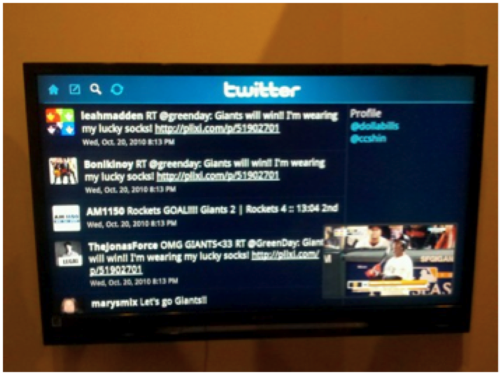
\includegraphics[width=6in]{images/googletv.png}
%\caption{Twitter on GoogleTV} \label{fig:google}
%\end{center}
%\end{figure} 
